%!TEX root = ./presentation.tex

\section{Einleitung}
\begin{frame}{Inhaltsverzeichnis}
\tableofcontents[currentsection]
\end{frame}


%-----------------------------------------------------------

\section{Einleitung}
\begin{frame}{\insertsectionhead}
	\begin{itemize}
		\item Ergänzung zu Masterarbeit: Rentabilität einer Solaranlage
		\item Früher: Erlös $>$ eigene Kosten
		\item Jetzt: Erlös $<$ eigene Kosten
		\item Frage: Wie hoch wann Stromverbrauch, wann Amortisierung?
	\end{itemize}
\end{frame}

%-----------------------------------------------------------
\begin{frame}{Aufgabe}
\begin{itemize}
	\item Interpolation von Werten
	\item Prognosen für weitere Werte
	\item Schätzen von weiteren Daten anhand Profils
	\bigskip
	\item Daten: 2 Lastgänge im Excel Format (2016 \& 2017):
	
\begin{table}[]
	\begin{tabular}{lllll}
		& Datum    & Uhrzeit & Wert [kWh] &  \\
		& 01.01.16 & 00:15   & 0,228      &  \\
		& 01.01.16 & 00:30   & 0,211375   &  \\
		& 01.01.16 & 00:45   & 0,192375   & 
	\end{tabular}
\end{table}
	
\end{itemize}
\end{frame}

%-----------------------------------------------------------
\begin{frame}{Einleitung (bessere Überschrift finden)}
\begin{itemize}
	\item Daten aus Excel Dokument extrahieren
	\item Daten in geeignete Datentypen konvertieren
	\item Daten für Visualisierung vorbereiten
	\begin{itemize}
		\item Hilfsmatrizen
		\begin{itemize}
			\item Stündlich
			\item Täglich
			\item Monatlich
		\end{itemize}
		\item Anpassungen
	\end{itemize}
\end{itemize}
\end{frame}


%-----------------------------------------------------------

\section{Algorithmen}
\begin{frame}{Inhaltsverzeichnis}
\tableofcontents[currentsection]
\end{frame}

%-----------------------------------------------------------
\subsection{Korrelationsmatrix}
\begin{frame}{\insertsubsectionhead}
	%TBC..
	%Eingabe: mList = durchschnittliche Monatshilfsmatrix
	%Ausgabe: aList = Korrelationsmatrix
	
    %mList = outlier(mList)
    %\right) mList = outlier(mList)

\end{frame}

%-----------------------------------------------------------
\subsection{Lineare Interpolation}
\begin{frame}{\insertsubsectionhead}
\begin{figure}
  \centering
     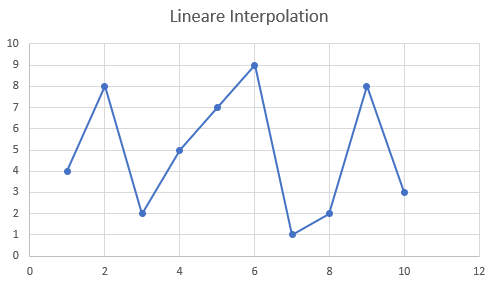
\includegraphics[width=0.5\textwidth]{pics/linear.png}
  %\tiny{\caption{Übersicht der Bestandteile}}
  \label{fig:Bild1}
\end{figure}
\begin{itemize}
\item Verfahren legt eine Gerade zwischen zwei Punkte $x_1$ \& $x_2$
\item Gesuchte Werte liegen auf der Geraden
\item Für jeden unbekannten Datenpunkt $P(x/y)$ gilt:
$$y = y_1 + \frac{y_2 - y_1}{x_2 - x_1} \cdot (x - x_1)$$
mit $x1\leq\ $x $\leq \ x_2$
\item Erzeugt stetigen, aber keinen glatten Verlauf der Funktion
\end{itemize}
\end{frame}

%-----------------------------------------------------------
\subsection{Polynomielle Interpolationsverfahren}
\begin{frame}{\insertsubsectionhead}
\begin{figure}
  \centering
     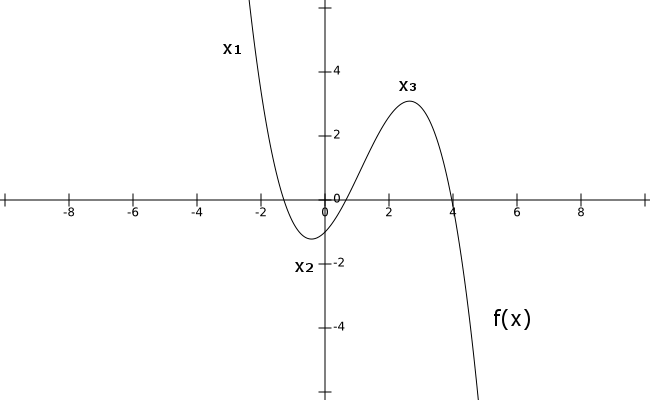
\includegraphics[width=0.7\textwidth]{pics/polynoms.png}
  %\tiny{\caption{Übersicht der Bestandteile}}
  \label{fig:Bild1}
\end{figure}
\begin{itemize}
\item Versuchen, durch gegebene Punkte eine Kurve zu legen
\item Finden zu $n+1$ paarweise verschiedenen Datenpunkten ein Interpolationspolynom maximal $n-ten$ Grades
\end{itemize}
\end{frame}

%-----------------------------------------------------------
\begin{frame}{Interpolationsverfahren nach Newton (1/2)}
\begin{block}{Vorgehensweise}
\begin{itemize}
\item Gegeben sind n Stützstellen
\item Annäherung an die Polynomfunktion vom möglichst kleinen Grad an (bis Grad $n$)
\item Gesucht: Polynomfunktion für $n+1$ Stützstellen
\begin{itemize}
\item Mit unbekannten Verbrauchsdaten bei $n+1$
\end{itemize}
\end{itemize}
\end{block}
\begin{block} {Interpolationspolynom}
\underline{Formel}
\begin{itemize}
\item $p_n(x) = a_0+a_1(x_n-x_0)+...+a_n(x_n-x_0)(x_n-x_1)...(x_n-x_{n-1})$
\item Für $n+1$ wird die Formel nach diesem Schema erweitert
\end{itemize}
\end{block}
\end{frame}

%-----------------------------------------------------------
\begin{frame}{Interpolationsverfahren nach Newton (2/2)}
\begin{block} {Charakteristika}
\underline{Vorteile}
\begin{itemize}
\item Polynom muss bei weiteren Punkten nicht komplett neu berechnet werden (vgl. Interpolation nach Lagrange)
\end{itemize}
\underline{Nachteile}
\begin{itemize}
\item Je größer der Grad, desto instabiler die Polynome (schwingen stark zwischen sehr verschiedenen Punkten)
\item \textit{Lösung 1:} Betrachtung der n nächsten Nachbarn
\item \textit{Lösung 2:} Verwendung eines alternativen Verfahrens
\end{itemize}
\end{block}
\end{frame}

%-----------------------------------------------------------
\begin{frame}{Splines}
\begin{block}{Ziel des Algorithmus}
\begin{itemize}
\item Finden von Stützstellen zwischen vorhandenen Datenpunkten
\item Jeder Teil des Splines ist durch eine Parabel mit geeigneten Koeffizienten definiert, z.B. $a_{i}x^3 + b_{i}x^2 + c_{i}x + d_{i}$
\begin{itemize}
\item Heraus kommt eine Funktion niedrigen Grades
\item Interpolation wird stückweise vorgenommen
\end{itemize}
\end{itemize}
\end{block}
\begin{block} {Charakteristika}
\underline{Vorteile}
\begin{itemize}
\item Linearer Rechenaufwand
\item Polynome werden nicht zunehmend instabiler
\end{itemize}
\underline{Nachteile}
\begin{itemize}
\item Können keine Verbrauchswerte in der Zukunft vorhersagen
\end{itemize}
\end{block}
\end{frame}

%-----------------------------------------------------------
\subsection{\grqq Intelligente\grqq Interpolationsverfahren}
\begin{frame}{\insertsubsectionhead}
\begin{itemize}
\item Wie sehr eignen sich rein mathematische Betrachtungen für die Interpolation?
\begin{itemize}
\item Energieverbrauch unterliegt keinem Funktionsgraphen
\item Es können auch unrealistisch hohe oder niedrige Werte auftreten
\end{itemize}
\item \underline{Neuer Schwerpunkt:} Interpolation ausschließlich auf Basis realer Daten
\end{itemize}
\end{frame}

%-----------------------------------------------------------
\begin{frame}{Interpolation aus Daten vom Vortag (1/2)}
\begin{block}{Idee}
\begin{itemize}
\item Tagesabläufe unterliegen meistens einem bestimmten Schema
\begin{itemize}
\item Energieverbrauch ändert sich nicht stark vom vorherigen Tag
\item Mo-Fr und Sa-So/Feiertage zeigen ähnliche Verbrauchsverläufe
\end{itemize}
\item Wenn ein Verbrauchswert fehlt, wird der Wert des Vortages genommen (gleiche Uhrzeit)
\item Weniger Rechenaufwand \& Ergebnisse orientieren sich näher an realem Verbrauchsverhalten
\end{itemize}
\end{block}
\end{frame}

%-----------------------------------------------------------
\begin{frame}{Interpolation aus Daten vom Vortag (2/2)}
\begin{figure}
  \centering
     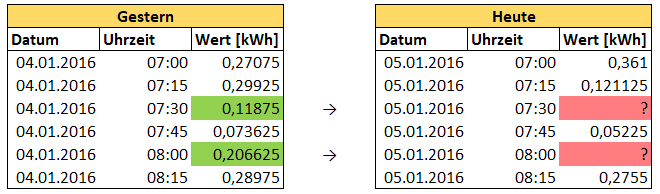
\includegraphics[width=0.75\textwidth]{pics/yesterday2.png}
  %\tiny{\caption{Übersicht der Bestandteile}}
  \label{fig:Bild1}
\end{figure}
\begin{block}{Fehlerpotentiale}
\begin{itemize}
\item Den Personen wird ein geregelter Tagesablauf unterstellt
\item Es können versehentlich Peaks erfasst werden
\end{itemize}
\end{block}
\end{frame}

%-----------------------------------------------------------
\begin{frame}{Durchschnittsbildung}
\begin{block}{Idee}
\begin{itemize}
	\item Verallgemeinerung der Interpolation aus Daten vom Vortag
	\item Berechnung der Werte auf Basis anderer Daten in bestimmten Abständen
	\begin{itemize}
		\item Mögliche Abstände: Wochen, Tage, umliegende Werte
		\item Anzahl und Gewichtung pro Intervall definierbar
	\end{itemize}
\end{itemize}
\end{block}
\begin{block}{Herausforderungen}
\begin{itemize}
	\item Konfiguration der Intervalle und Gewichtungen
	\item Starke Einschränkungen bei der Interpolation großer Lücken
\end{itemize}
\end{block}
\end{frame}

%-----------------------------------------------------------
\begin{frame}{Datenbankansatz (1/2)}
\begin{block}{Idee}
\begin{itemize}
	\item Interpolation nicht nur aus den (lückenhaften) zur Verfügung gestellten Daten
	\item Bildung einer Datenbasis aus Lastprofilen vieler Haushalte
	\item Kategorisierung der Datensätzen
	\begin{itemize}
		\item Einfache Beschreibungen (Wohnung / Haus, etc.)
		\item Numerische Einordnung (Personenanzahl, Wohnfläche, etc.)
	\end{itemize}
	\item Interpolation nur aus "ähnlichen" Datensätzen
	\begin{itemize}
		\item Filterung auf Basis der Kategorisierung
		\item Durchschnittsbildung der gefilterten Datensätze
		\item Erweiterung: gewichteter Durchschnitt, Anpassung an umliegende Werte in lückenhaftem Datensatz
	\end{itemize}
	\item Speicherung in andersartigem Datenformat - Unabhängigkeit von Erfassungsjahr
\end{itemize}
\end{block}
\end{frame}

%-----------------------------------------------------------
\begin{frame}{Datenbankansatz (2/2)}
\begin{block}{Vorteile}
\begin{itemize}
	\item Interpolation ohne eigene Daten oder für lückenhafte Daten
	\item Einfluss vieler Datensätze führt zu sehr realistischen Ergebnissen
	\item Granulare Konfiguration des eigenen Haushalts möglich
\end{itemize}
\end{block}
\begin{block}{Nachteile}
\begin{itemize}
	\item Große Datenbasis erforderlich
	\item Zusätzliche Kategorisierung
\end{itemize}
\end{block}
\end{frame}

%-----------------------------------------------------------
\section{Heuristiken}
\begin{frame}{Inhaltsverzeichnis}
\tableofcontents[currentsection]
\end{frame}

%-----------------------------------------------------------
\subsection{Feiertage}
\begin{frame}{\insertsubsectionhead}
\begin{block}{Wie sollen Feiertage interpoliert werden?}
\begin{itemize}
\item Der Datentyp LocalDateTime kann Wochentage erfassen, aber keine Feiertage
\item Es gibt in Java keine guten Libraries für Feiertage
\item \underline{Welche Feiertage werden benötigt?}
\begin{itemize}
\item Ändern sich je nach Land und Bundesland/Region
\item Was ist mit Personen, die pendeln?
\end{itemize}
\end{itemize}
\end{block}
\begin{block}{Implementierung im Programm}
\begin{itemize}
\item Manueller Import von iCalendar-Dateien (standardisiertes Dateiformat)
\end{itemize}
\end{block}
\end{frame}

%-----------------------------------------------------------
\subsection{Mustererkennung}
\begin{frame}{\insertsubsectionhead}
\begin{block}{Bildung von Intervallen}
\smallskip
\small{Beispiel mit Intervallgröße 4: [00:00-03:39Uhr],[04:00-07:59Uhr]...}\normalsize
\smallskip
\begin{itemize}
\item Ermittlung folgender Werte:
\begin{itemize}
\item Durchschnittsverbrauch pro Intervall
\item Globaler Durchschnittsverbrauch
\end{itemize}
\end{itemize}
\end{block}
\begin{block}{Detektion von Interpolations-Ausreißern}
\begin{itemize}
\item Durchschnittswerte geben Auskunft darüber, wann eine Person bspw. schläft oder wann sie viele Geräte benutzt
\item Interpolierte Werte werden mit Durchschnittsverbrauchen verglichen
\end{itemize}
\end{block}

\end{frame}


%-----------------------------------------------------------
\begin{frame}{Stromverbrauch der Haushalte}
\begin{figure}
  \centering
     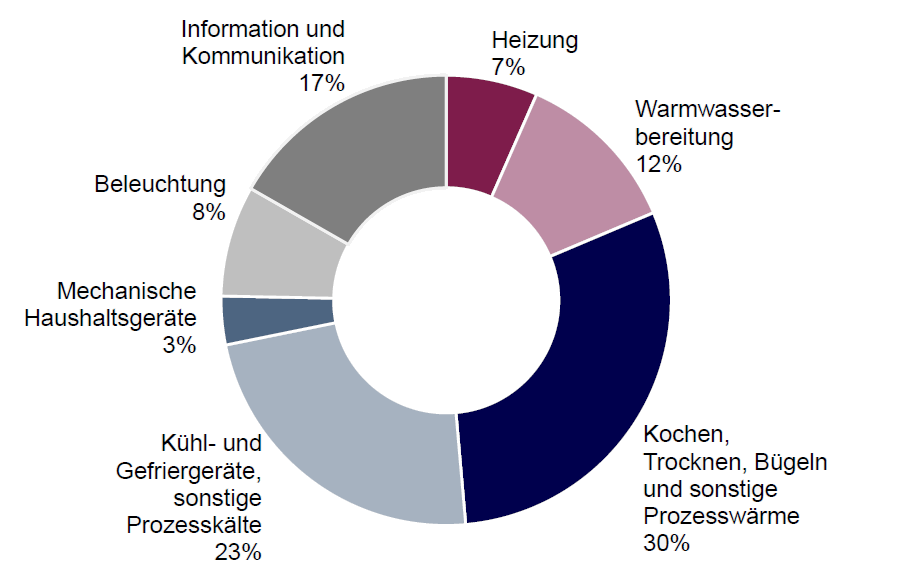
\includegraphics[width=0.9\textwidth]{pics/avgEnergyConsumption.png}
  	\caption{Struktur des Stromverbrauchs nach Anwendungsbereichen 2016 \cite{bdew:consumption}}
  \label{fig:Bild1}
\end{figure}
\end{frame}

%-----------------------------------------------------------
\subsection{Durchschnittlicher Tages-\& Nachtverbrauch}
\begin{frame}{\insertsubsectionhead}
\begin{block}{Wann geeignet?}
\begin{itemize}
\item Wenn sehr viele Verbrauchsdaten fehlen
\end{itemize}
\end{block}
\begin{block}{Die Heuristik bedient sich folgender Elemente}
\begin{itemize}
\item Berechnung des durchschnittlichen Tages-/Stundenverbrauchs auf Basis von:
\begin{itemize}
\item Anteiliger Verbrauch der Geräte
\item Anzahl der Personen im Haushalt
\end{itemize}
\item Durchschnittliche Ruhezeiten
\begin{itemize}
\item werktags
\item an Wochenenden und Feiertagen
\end{itemize}
\item Anwendung auf interpolierte Werte, die sich stark vom durchschnittlichen Wertebereich unterscheiden
\end{itemize}
\end{block}
\end{frame}

%-----------------------------------------------------------
\subsection{Saisonaler Verbrauch}
\begin{frame}{\insertsubsectionhead}
\begin{block}{Einfluss der Jahreszeiten}
\begin{itemize}
\item Höherer Verbrauch im Winter als im Sommer
\item Nachträgliche Berücksichtigung in den interpolierten Werten
\begin{itemize}
\item Verspricht vor allem einen Nutzen für die rein mathematischen Algorithmen oder für mehrere fehlende Monate im Datensatz
\end{itemize}
\end{itemize}
\end{block}
\begin{block}{Heuristiken}
\begin{itemize}
\item $10\%$-Statistik vom Europäischen Fonds für regionale Entwicklung (EFRE)
\item Prozentsatz aus den vorhandenen Daten
\end{itemize}
\end{block}
\end{frame}

%-----------------------------------------------------------
\section{Evaluation \& Bewertung}
\begin{frame}{Inhaltsverzeichnis}
\tableofcontents[currentsection]
\end{frame}

%-----------------------------------------------------------
\begin{frame}{Evaluation \& Bewertung}
\begin{block}{Vorgehen}
\begin{itemize}
	\item Gegeben: ein vollständiger Datensatz
	\item Vorbereitung eines Testdatensatzes
	\begin{itemize}
		\item Zufälliges Entfernen bestimmter Elemente
		\item Konfigurierbarer zu entfernenden Anteil an Wochen, Tagen, Stunden und einzelnen Elementen
	\end{itemize}
	\item Durchführung der Interpolation
	\item Bewertung des Ergebnisses: Mittelwert der euklidischen Distanzen
	\item Manuelle Definition der Konfigurationsparameter
	\item Datenbankansatz nur mit Original als einzigem Element
\end{itemize}
\end{block}
\end{frame}

%-----------------------------------------------------------
\begin{frame}{Evaluation \& Bewertung}
\begin{block}{Algorithmen}
\begin{figure}
	\centering
	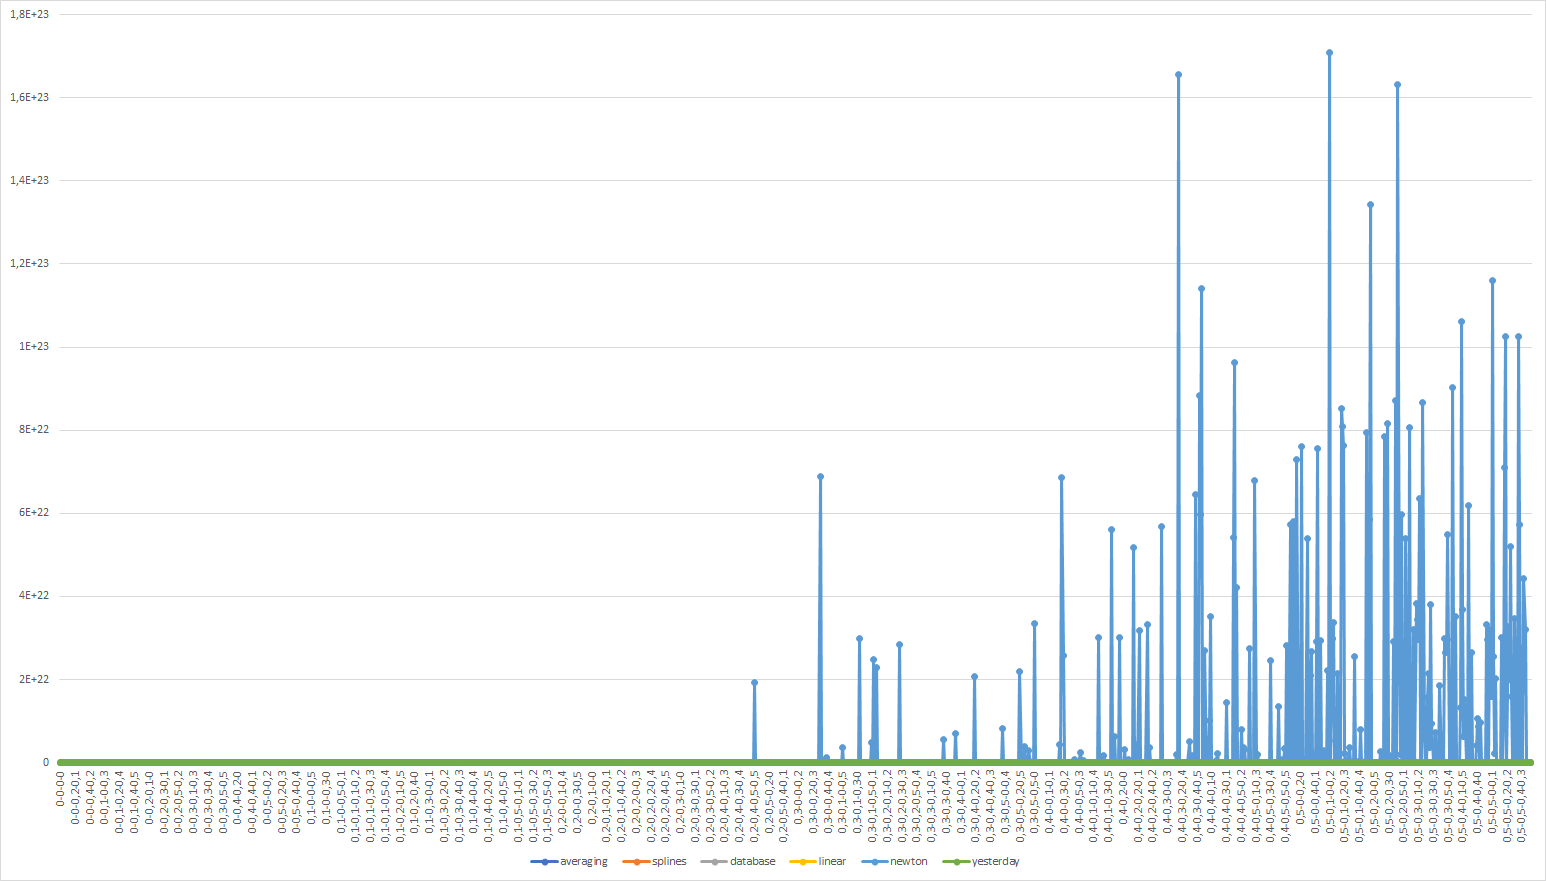
\includegraphics[width=1\textwidth]{pics/evaluation-algorithms-1.png}
	\caption{Gesamtergebnisse}
%	\label{fig:Bild1}
\end{figure}
\end{block}
\end{frame}

%-----------------------------------------------------------
\begin{frame}{Evaluation \& Bewertung}
\begin{block}{Algorithmen}
\begin{itemize}
	\item Newton liefert gute Ergebnisse, wenn Lücken weniger als ein Tag lang sind
\end{itemize}
\end{block}
\end{frame}

%-----------------------------------------------------------
\begin{frame}{Evaluation \& Bewertung}
\begin{block}{Algorithmen}
\begin{figure}
	\centering
	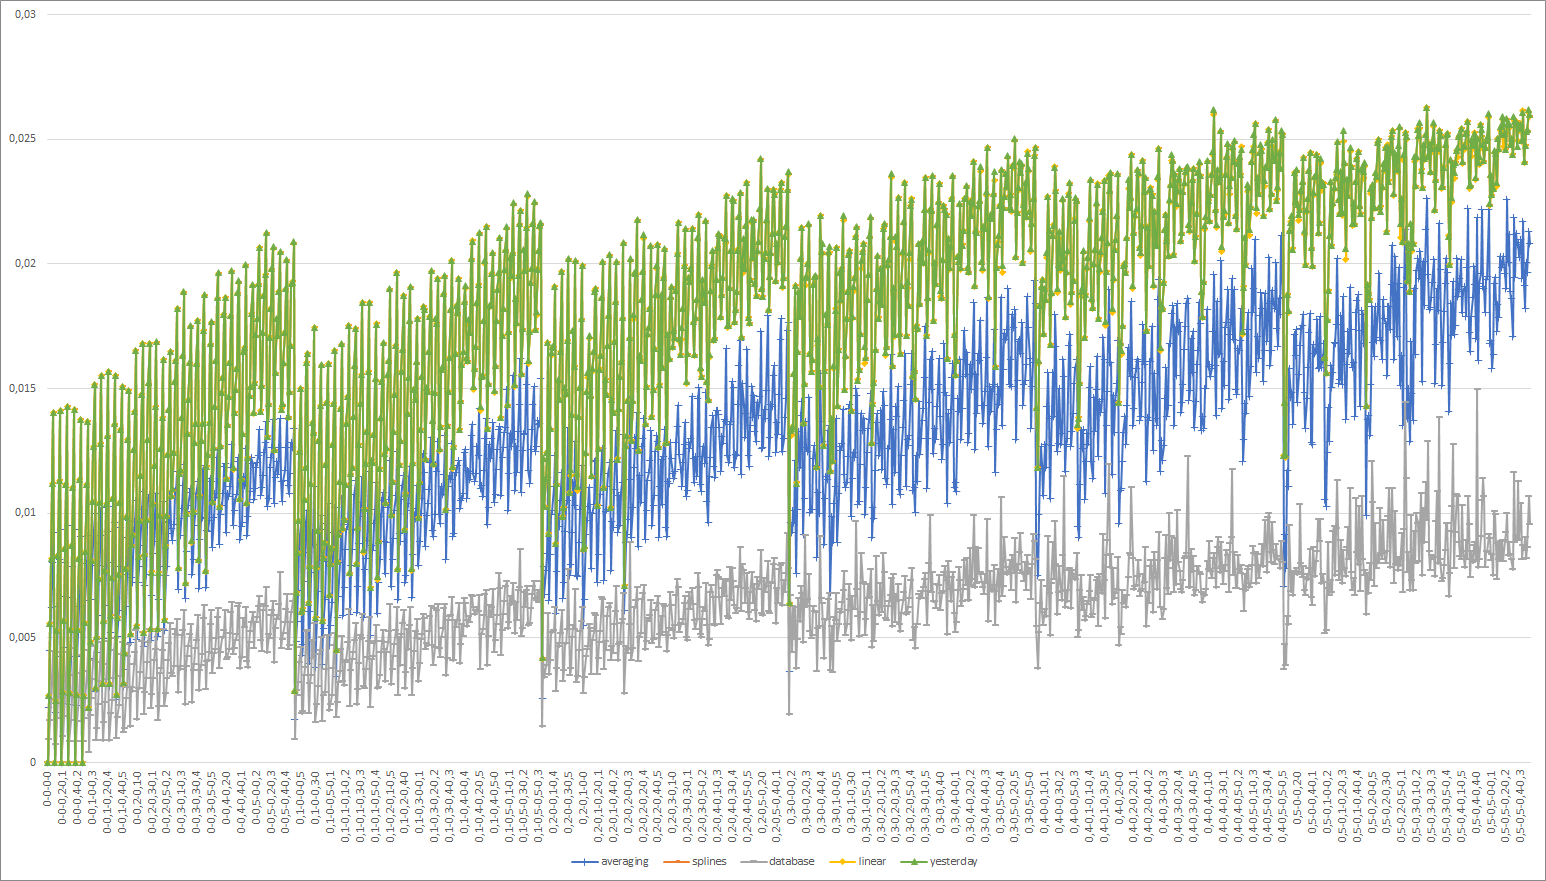
\includegraphics[width=1\textwidth]{pics/evaluation-algorithms-2.png}
	\caption{Gesamtergebnisse ohne Newton}
	%	\label{fig:Bild1}
\end{figure}
\end{block}
\end{frame}

%-----------------------------------------------------------
\begin{frame}{Evaluation \& Bewertung}
\begin{block}{Algorithmen}
\begin{itemize}
	\item Newton liefert gute Ergebnisse, wenn Lücken weniger als ein Tag lang sind
	\item Sehr ähnliche Ergebnisse für Yesterday, Linear und Splines
	\item Bessere Ergebnisse für Averaging
	\item Bestes Ergebnis für Datenbankansatz
\end{itemize}
\end{block}
\end{frame}

%-----------------------------------------------------------
\begin{frame}{Evaluation \& Bewertung}
\begin{block}{Algorithmen}
\begin{figure}
	\centering
	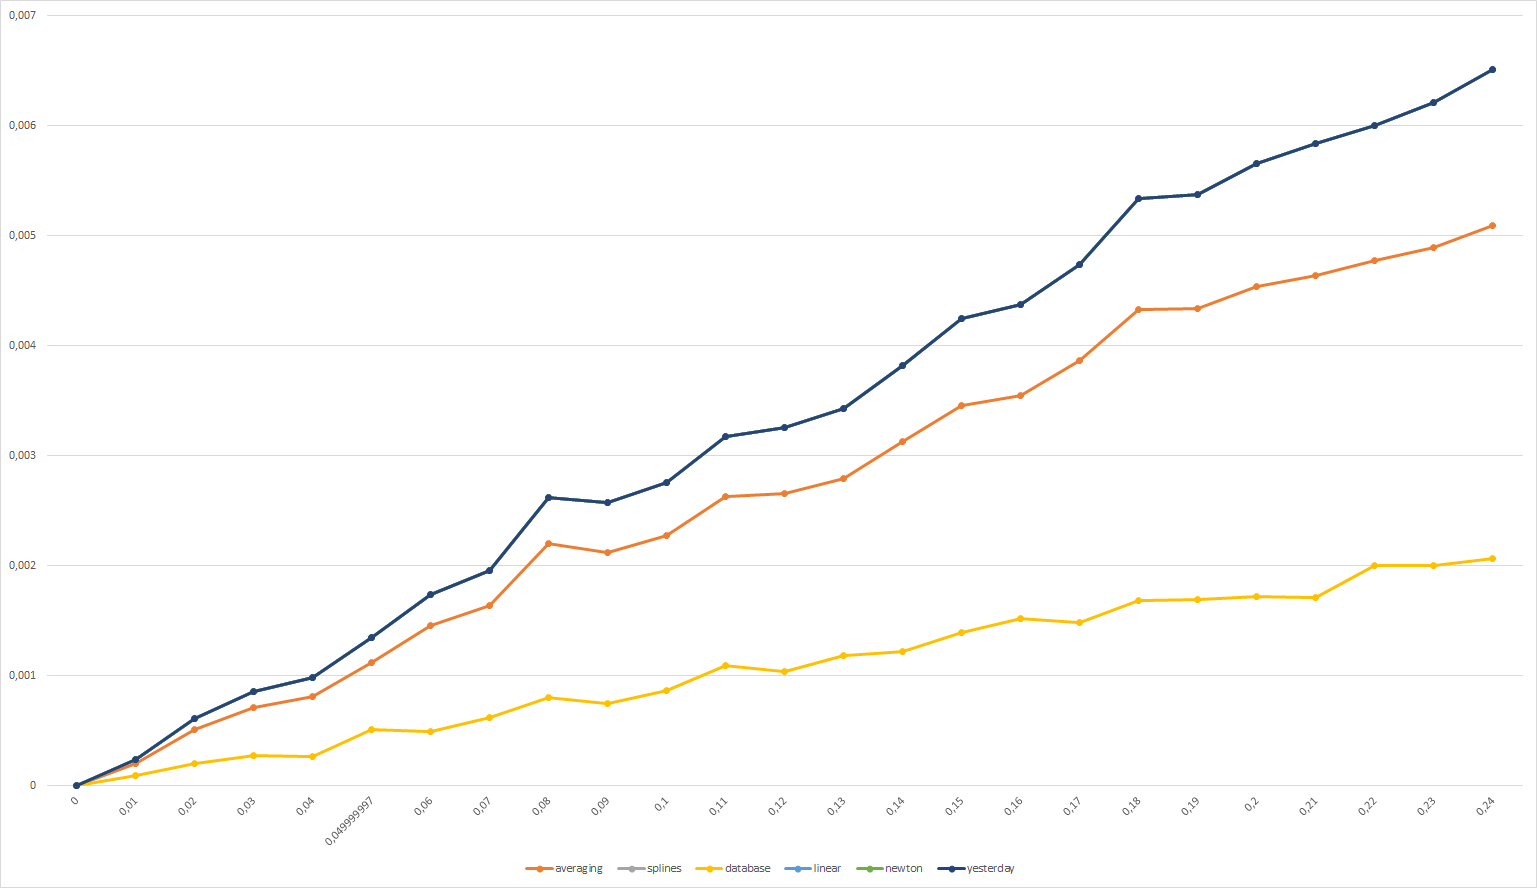
\includegraphics[width=1\textwidth]{pics/evaluation-algorithms-3.png}
	\caption{Ergebnisse nur mit einzelnen fehlenden Elementen}
	%	\label{fig:Bild1}
\end{figure}
\end{block}
\end{frame}

%-----------------------------------------------------------
\begin{frame}{Evaluation \& Bewertung}
\begin{block}{Heuristiken}
\begin{figure}
	\centering
	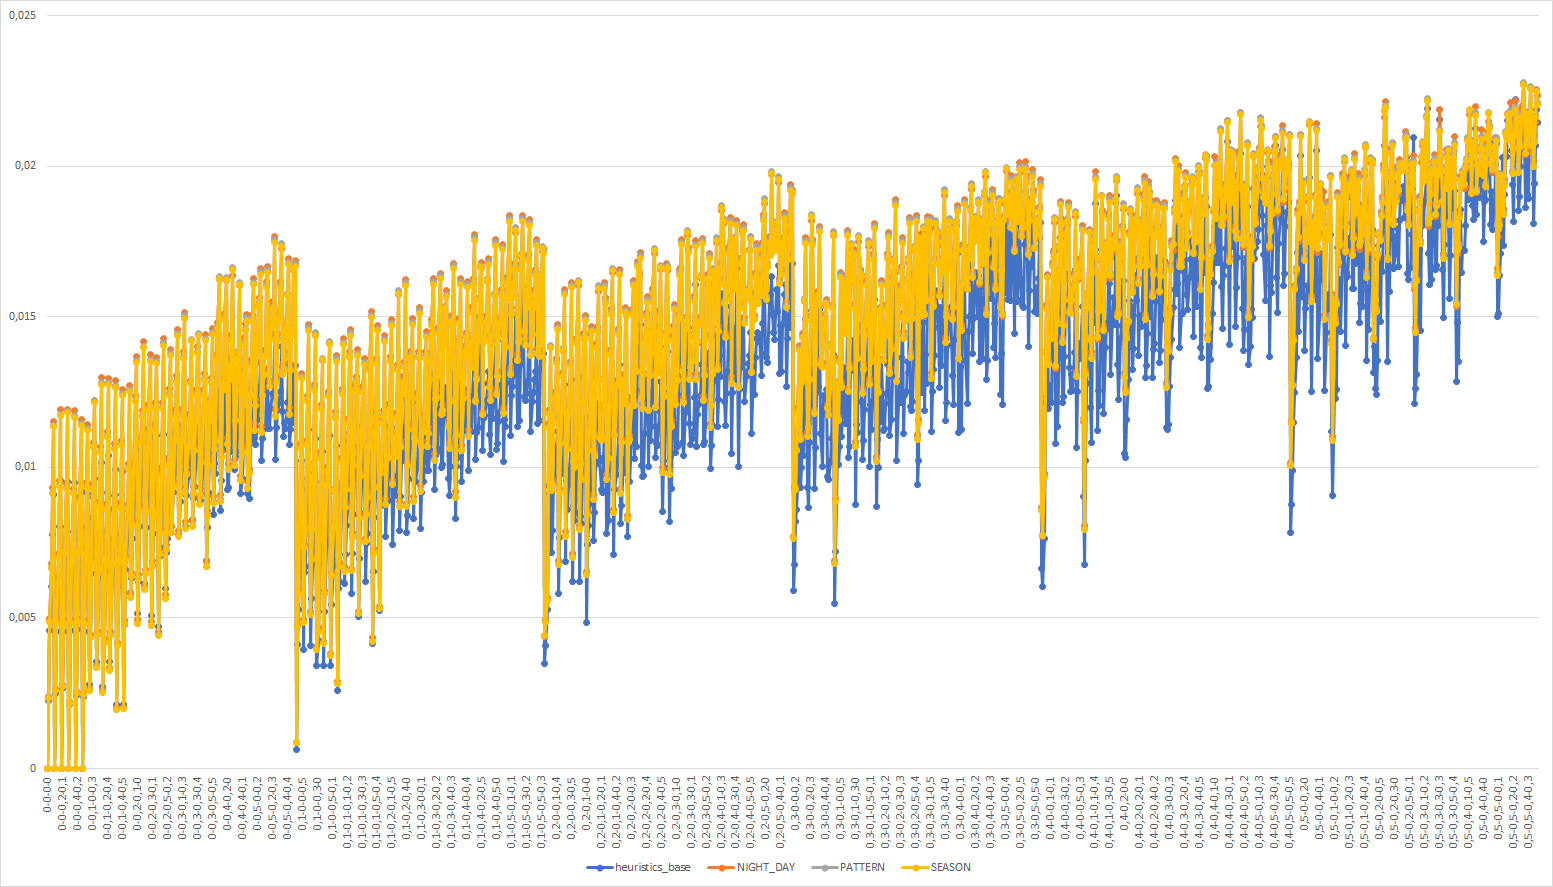
\includegraphics[width=1\textwidth]{pics/evaluation-heuristics.png}
	\caption{Ergebnisse nur mit einzelnen fehlenden Elementen}
	%	\label{fig:Bild1}
\end{figure}
\end{block}
\end{frame}

%-----------------------------------------------------------
\begin{frame}{Evaluation \& Bewertung}
\begin{block}{Heuristiken}
\begin{itemize}
	\item Sehr ähnliche Werte für alle Heuristiken
	\item Mit dieser Konfiguration Verschlechterung der Ergebnisse
\end{itemize}
\end{block}
\end{frame}

%-----------------------------------------------------------
\section{Ausblick}
\begin{frame}{Inhaltsverzeichnis}
\tableofcontents[currentsection]
\end{frame}

%-----------------------------------------------------------
\begin{frame}{Ausblick}
\begin{itemize}
	\item Verbesserung der Ergebnisse mit großer Datenmenge
	\item Bestimmung der Konfigurationsparameter verbessern
	\begin{itemize}
		\item Tieferes Fachwissen
		\item Lernen von Parametern durch Optimierung
	\end{itemize}
	\item Einsatz komplexerer Algorithmen
\end{itemize}
\end{frame}
